%%%%%%%%%%%%%%%%%%%%%%%%%%%%%%%%%%%%%%%%%
% fphw Assignment
% LaTeX Template
% Version 1.0 (27/04/2019)
%
% This template originates from:
% https://www.LaTeXTemplates.com
%
% Authors:
% Class by Felipe Portales-Oliva (f.portales.oliva@gmail.com) with template 
% content and modifications by Vel (vel@LaTeXTemplates.com)
%
% Template (this file) License:
% CC BY-NC-SA 3.0 (http://creativecommons.org/licenses/by-nc-sa/3.0/)
%
%%%%%%%%%%%%%%%%%%%%%%%%%%%%%%%%%%%%%%%%%

%----------------------------------------------------------------------------------------
%	PACKAGES AND OTHER DOCUMENT CONFIGURATIONS
%----------------------------------------------------------------------------------------

\documentclass[
	12pt, % Default font size, values between 10pt-12pt are allowed
	%letterpaper, % Uncomment for US letter paper size
	%spanish, % Uncomment for Spanish
]{fphw}

% Template-specific packages
\usepackage[utf8]{inputenc} % Required for inputting international characters
\usepackage[T1]{fontenc} % Output font encoding for international characters
\usepackage{mathpazo} % Use the Palatino font

\usepackage{graphicx} % Required for including images

\usepackage{booktabs} % Required for better horizontal rules in tables

\usepackage{listings} % Required for insertion of code

\usepackage{enumerate} % To modify the enumerate environment

%----------------------------------------------------------------------------------------
%	ASSIGNMENT INFORMATION
%----------------------------------------------------------------------------------------

\title{Homework \#1} % Assignment title

\author{Karamveer Kaur} % Student name

\date{August 2nd,2019} % Due date

\institute{University of Concordia \\ Department of software engineering} % Institute or school name

\class{Software Engineering Process} % Course or class name

\professor{Dr. Pankaj Kamthan} % Professor or teacher in charge of the assignment

%----------------------------------------------------------------------------------------

\begin{document}

\maketitle % Output the assignment title, created automatically using the information in the custom commands above

%----------------------------------------------------------------------------------------
%	ASSIGNMENT CONTENT
%----------------------------------------------------------------------------------------

\section*{Question 5}
\subsection*{Function1}
\subsection*{F1 By Shashank Rao}

%------------------------------------------------

%----------------------------------------------------------------------------------------



\begin{problem}
  Code Review
\end{problem}

%------------------------------------------------
\item 1. GUI is highly coupled with the business logic.
\item 2. Functions are lengthy.
\item 3. Code is working fine.
\item 4. JavaDocs are maintained.
\item 5. No severe violations found by checkstyle.
\item 6. Code is somewhat adherent to coding standards.
\item 7. No Compilation error.
\begin{center} 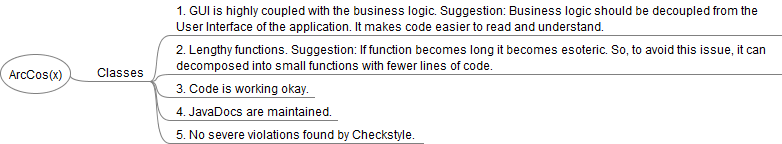
\includegraphics[width=0.5\columnwidth]{CodeReview.png} % Example image 
\end{center}


%----------------------------------------------------------------------------------------

\section*{Approach of review}

\begin{problem}
	Step by step approach to review the source code
	
\end{problem}

%------------------------------------------------

\subsection*{Answer}
Step by step process
\begin{center} 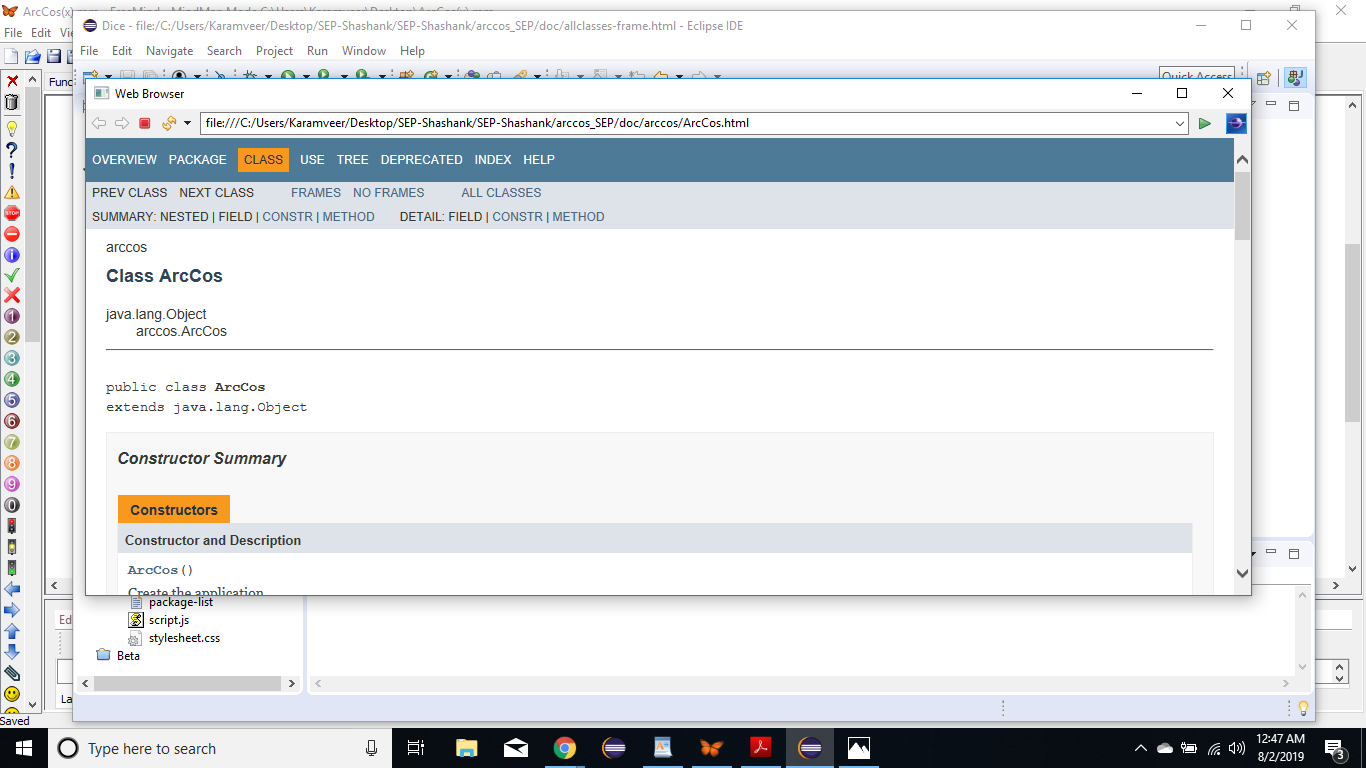
\includegraphics[width=0.5\columnwidth]{ShashankJavaDoc.png} % Example image 
\end{center}
\item 1.Installation of Free Mind
\item 2.Importing the project into Free Mind
	\begin{enumerate}[(\itshape a\normalfont)] % Sub-questions styled as italic letters
		\item Setting up the environment.
		\item Installed jacoco to check code coverage.
		\item Installed Checkstyle plugin.
		\begin{center} 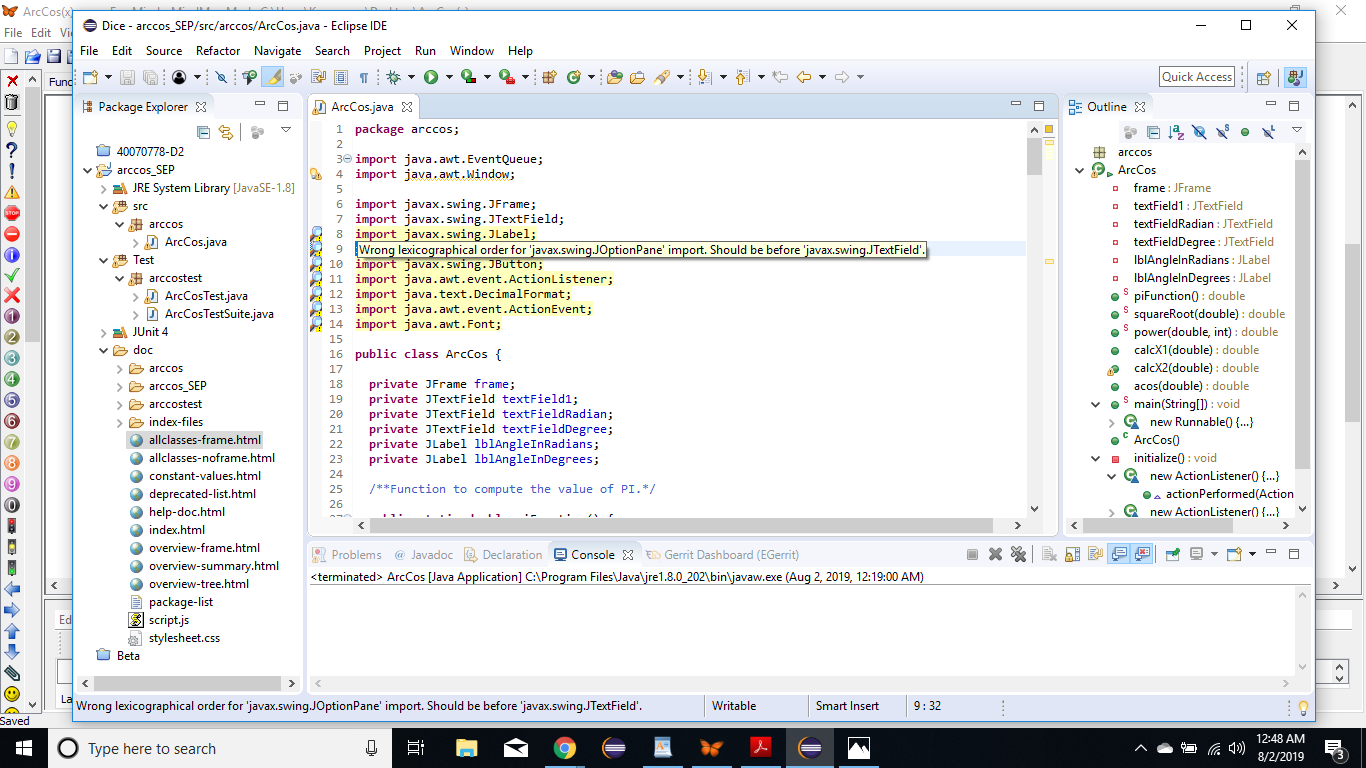
\includegraphics[width=0.5\columnwidth]{ShashankCheckstyle.png} % Example image 
\end{center}
        \item Setting up of Gerrit plugin.
	\end{enumerate}
\item 3.Read the code Manually.
\item 4.Checked if it is adhered to coding conventions.
\item 5.Checked for java doc.
\item 5.Testing if code is working properly.
\item 6.Suggestions given accordingly.
%-------------------------------------------

%----------------------------------------------------------------------------------------

\section*{Question 7}
\subsection*{Function9}
\subsection*{F9 By Sneha Sarkar}
\begin{problem}
	Review of Test cases
\end{problem}
\begin{center} 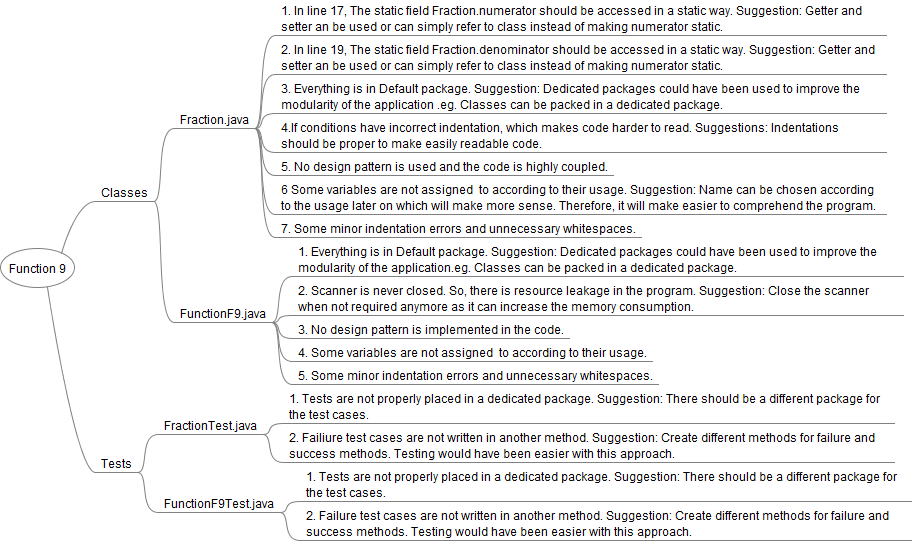
\includegraphics[width=0.5\columnwidth]{Function9Sarkar.png} % Example image 
\end{center}
\item 1.Proper package could be specified for test cases.
\begin{center} 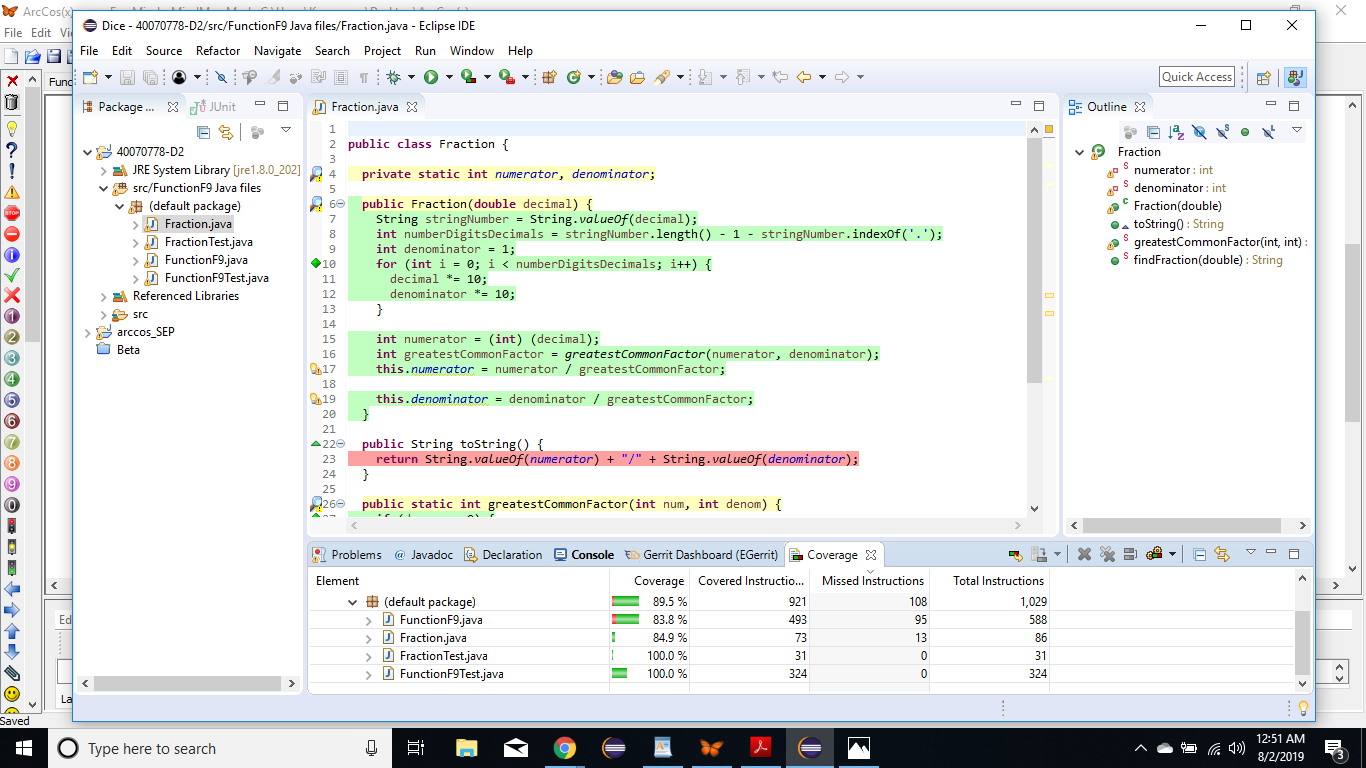
\includegraphics[width=0.5\columnwidth]{SarkarDefaultP.png} % Example image 
\end{center}
\item 2.Different method could be created to write failure test cases and success test cases.
\item 3.Instead of default package,dedicated package could be good approach.
\item 4.No compilation error
\item 5.Resource leakage should have been properly handled.
\item 6.Indentations were not appropriate according to conventions which makes code harder to read.

%------------------------------------------------

\begin{problem}
Step by step process
\end{problem}
\item 1.Installation of Free Mind
\item 2.Importing the project into Free Mind
	\begin{enumerate}[(\itshape a\normalfont)] % Sub-questions styled as italic letters
		\item Setting up the environment.
		\item Installed jacoco to check code coverage.
		\begin{center} 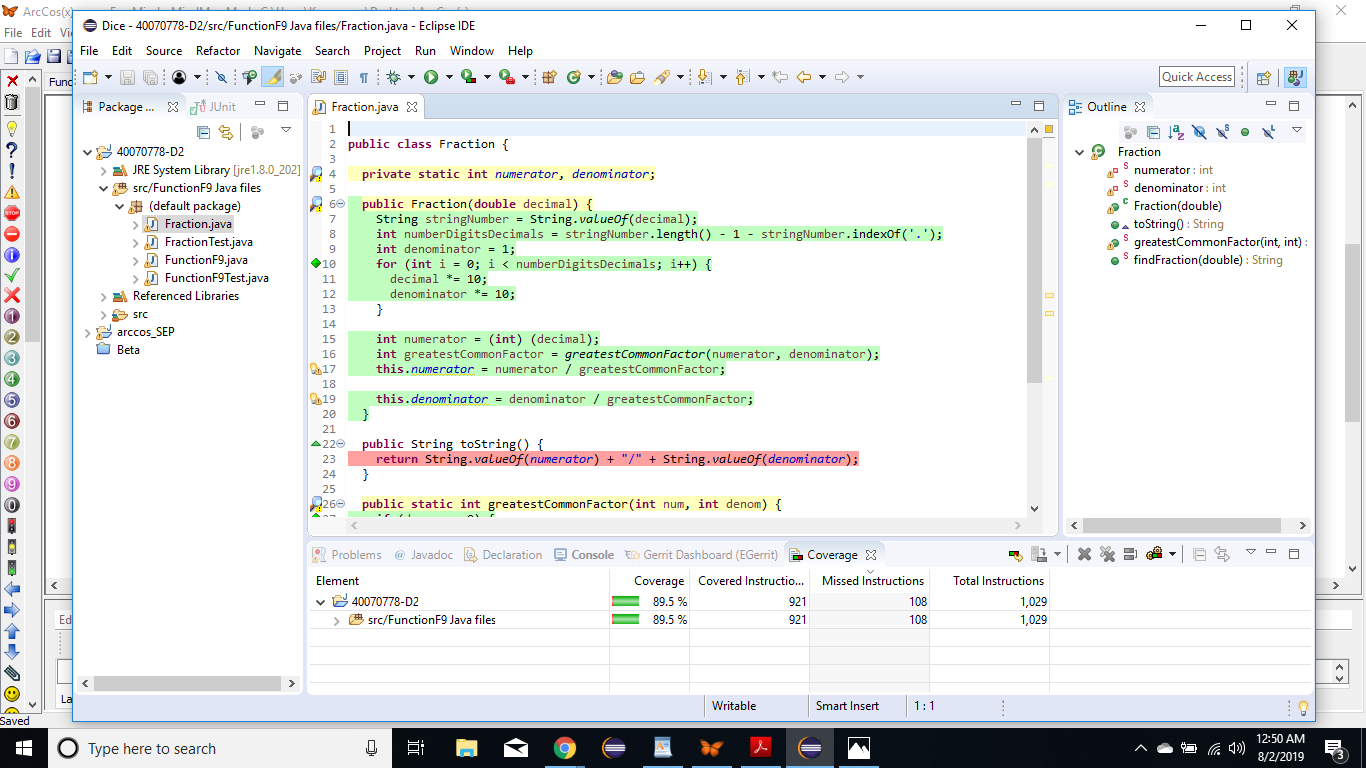
\includegraphics[width=0.5\columnwidth]{JacocoSarkar.png} % Example image 
\end{center}
	\end{enumerate}

\item 3.Read the code Manually.
\item 5.Testing if code is working properly by running test cases as well as manual testing.
\item 6.Suggestions given accordingly.
%----------------------------------------------------------------------------------------
\section{GitHub Repository}
https://github.com/karamveer28/soen-6011-project
\section{References}
https://phauer.com/2018/code-review-guidelines/
\newline
https://sourceforge.net/projects/freemind/
\newline
https://checkstyle.sourceforge.io/
\newline
https://www.eclemma.org/jacoco/
\newline
https://www.gerritcodereview.com/
\newline
\end{document}
